
% moved to appendix; no longer necessary
\part{Discrete Mathematics} % All of this part comes from Rosen's Discrete Mathematics and its Applications, Seventh Edition.
\thispagestyle{empty}
This is the part of this text which won't focus on numbers.
Were it not for specific examples, no numbers would exist in this part altogether.
If you've ever wondered why mathematicians are so hellbent on semantics, this will tell you why.
This part sets the stage for the logical theory behind mathematics.
\setcounter{section}{0}
\chapter{Propositional Logic}
\epigraph{This is your last chance. After this, there is no turning back. You
take the blue pill - the story ends, you wake up in your bed and believe
whatever you want to believe. You take the red pill - you stay in Wonderland and
I show you how deep the rabbit-hole goes.}{Morpheus, \emph{The Matrix}, 1999}
\label{ch:propositional}

The whole idea of propositional logic is that statements in mathematics have truth value and there is a logical process that we use to evaluate that truth value.
Perhaps most importantly, this chapter will introduce us to \emph{DeMorgan's Laws}, which are relevant everywhere from computer science (in simplifying boolean operators) to the writings of Aristotle.

\section{Introduction to Propositional Logic}
\label{sec:propintro}

\index{proposition}
  A \textbf{proposition} just a sentence that makes a statement.
  \begin{ex}
    ``My house is red.''
  \end{ex}

\index{propositional calculus}
  \textbf{Propositional calculus} (or \emph{propositional logic}) assigns propositions \emph{propositional variables}
  (e.g. \(p, q, r, s, \ldots\)) and deals with their logic and \emph{truth value}.
  \begin{ex}
    Let $p$ be ``my house is red.''
  \end{ex}

\index{negation}
  Let \(p\) be a proposition. The \textbf{negation} of \(p\), denoted by \[\neg p\] is the statement
  ``it is not the case that \(p\).''
  The truth value of \(\neg p\) is the opposite of the truth value of \(p\).
  \begin{ex}
    Let $p$ be ``my house is red.''

    Then $\neg p$ is ``it is not the case that my house is red,'' or simply ``my house is not red.''
  \end{ex}

\index{conjunction}
  Let \(p\) and \(q\) be propositions. The \textbf{conjunction} of \(p\) and \(q\), denoted by \[ p \wedge q \] is the proposition
  ``\(p\) and \(q\).'' It is true when both \(p\) and \(q\) are true and false otherwise.
  \begin{ex}
    Let $p$ be ``Kevin likes Sarah'' and let $q$ be ``Sarah likes Kevin.'

    Then $p \wedge q$ is ``Kevin likes Sarah and Sarah likes Kevin,'' or ``Kevin and Sarah like each other.''
    This statement would be false if either of the two did not like the other.
  \end{ex}

\index{disjunction}
  Let \(p\) and \(q\) be propositions. The \textbf{disjunction} of \(p\) and \(q\), denoted by \[ p \vee q \] is the proposition
  ``\(p\) and \(q\).'' It is true when either \(p\) or \(q\) are true and false otherwise.
  \begin{ex}
    Let $p$ denote ``Kevin hates bagels'' and $q$ denote ``Kevin hates poppy seeds.''

    The proposition $p \vee q$ is the statement ``Kevin hates bagels or poppy seeds.''
    Note, here, that there is an implicit cue in the language that Kevin could, indeed, hate both bagels and poppy seeds.
    The statement would be true if he were distasteful toward either one of them, or both.
  \end{ex}

\index{exclusive or}
  The \textbf{exclusive or} of \(p\) and \(q\), denoted by \[p \oplus q\] is true when exactly one of \(p\) and \(q\) is true and false otherwise.
  \begin{ex}
    Let $p$ mean ``I could sleep in all day today'' and $q$ mean ``I could go to work.''

    The statement $p \oplus q$ is true when only one of $p$ or $q$ is true.
    It is the sentence ``I could go to work, or I could sleep in all day today.''
    Since it does not make sense to do both at once, the \emph{exclusive or} is implied in our use of the English language.

    We should keep an eye out for this distinction between disjunciton and exclusive or, as it requires careful
    attention to the subtleties in our use of language.
  \end{ex}

  \index{conditional statement}
  The \textbf{conditional statement} \[p \implies q\] is the propsition ``if p, then q.''
  The conditional statement \(p \implies q\) is false when \(p\) is true and \(q\) is false, and true otherwise.
  Other ways of writing the conditional statement can be found in table \ref{tab:conditionals}.
  \index{hypothesis}\index{antecedent}\index{premise}
  \(p\) is called the \textbf{hypothesis} (or antecedent or premise).
  \index{conclusion}\index{consequence}
  \(q\) is called the \textbf{conclusion} (or consequence).
  \begin{ex}
    Let $p$ be ``Joe broke his arm'' and $q$ be ``Joe will go to the hospital.''

    The statement $p \implies q$ is the statement ``If Joe broke his arm, then he will go to the hospital.''
    It is true if Joe only goes to the hospital, if he only breaks his arm, and if both events occur.
    The only situation in which it is false is if Joe breaks his arm, then does not go to the hospital.
  \end{ex}
  \begin{table}[H]
  \centering
  %\boxed{
    \begin{tabular}{p{2in} p{2in}}
      ``if \(p\), then \(q\)'' & ``\(p\) implies \(q\)'' \\
      ``if \(p\), \(q\)'' & ``\(p\) only if \(q\)'' \\
      ``\(p\) is sufficient for \(q\)'' & ``a sufficient condition for \(q\) is \(p\)'' \\
      ``\(q\) if \(p\)'' & ``\(q\) whenever \(p\)`` \\
      ``\(q\) when \(p\)'' & ``\(q\) is necessary for \(p\)'' \\
      ``a necessary condition for \(p\) is \(q\)'' & ``\(q\) follows from \(p\)'' \\
      ``\(q\) unless \(p\)''
    \end{tabular}
  %}
  \caption{Other ways of writing the conditional statement \(p \implies q\).}
  \label{tab:conditionals}
\end{table}
\index{converse}
  The \textbf{converse} of \(p \implies q\) is \(q \implies p\).

\index{contrapositive}\label{def:contrapositive}
  The \textbf{contrapositive} of
  \(p \implies q\)
  is
  \(\neg q \implies \neg p\).
  It is logically equivalent to
  \(p \implies q\).
  We can prove this with the following \emph{truth table}:
  \begin{table}[H]
    \centering
    \begin{tabular}{|>$c<$|>$c<$|>$c<$|>$c<$|}
      \hline
      p & q & p\implies q & \neg q \implies \neg p\\
      \hline
      0 & 0 & 1 & 1 \\
      0 & 1 & 1 & 1 \\
      1 & 0 & 0 & 0 \\
      1 & 1 & 1 & 1 \\\hline
    \end{tabular}
    \caption{A truth table for $p\implies q$ and $\neg q \implies \neg p$.}
    \label{tab:contrapositive}
  \end{table}
  A \textbf{truth table} can be used to demonstrate the logical relationships between statements.

  This property of contrapositives is especially useful when we are trying to prove a statement,
  as its contrapositive is often easier to prove than the statement itself.
  This subject is detailed further in \ref{sec:contrapositive}.

\index{inverse}
  The \textbf{inverse} of \(p \implies q\) is \(\neg p \implies \neg q\).
  It has the opposite truth value of the original statement.

  \index{biconditional statement}
  The \textbf{biconditional statement}, also called \emph{bi-implication}, for $p$ and $q$ is \[p \iff q.\] This is the statement
  ``\(p\) if and only if \(q\).''
  It is true when both \(p\) and \(q\) have the same truth value, and false otherwise.
\begin{table}[h]
  \centering
    \begin{tabular}{l}
      ``\(p\) is necessary and sufficient for \(q\)'' \\
      ``if \(p\), then \(q\), conversely'' \\
      ``p iff q''
    \end{tabular}
  \label{tab:biconditionals}
\end{table}
In mathematical theorems, definitions, and related elements later in this text, we will often see the biconditional operator written \emph{iff}.

\section{Logical Equivalence}
\index{tautology}
  A \textbf{tautology} is a compound proposition that is always true, regardless of the truth values of the variables that occur in it.
\index{contradiction}
  A \textbf{contradiciton} is a compound proposition that is always false.
\index{contingency}
  A \textbf{contingency} is a compound proposition that is nither a tautology nor a contradiction.
  It can be either true or false.
\begin{ex}
  \( p \iff q \) is logically equivalent to \( (p \implies q) \wedge (q \implies p)\).
  We state this by writing
  \[ p \leftrightarrow q \equiv (p \implies q) \wedge (q \implies p).\]
\end{ex}
\begin{table}  \centering
  \boxed{
    \begin{tabular}{>{\(}l<{\)} >{\(}r<{\)}|>{\(}c<{\)}|>\(c<\)|>\(c<\)|>\(c<\)}
      p & q & \neg q & p \lor \neg q & p \land q & (p \lor \neg q) \implies (p \land q) \\ \hline
      1 & 1 & 0 & 1 & 1 & 1 \\
      1 & 0 & 1 & 1 & 0 & 0 \\
      0 & 1 & 0 & 0 & 0 & 1 \\
      0 & 0 & 1 & 1 & 0 & 0
    \end{tabular}
  }
  \caption{The truth table for \((p \lor \neg q) \implies (p \land q)\)}
\end{table}
\index{logical equivalence}
The compound propositions \(p\) and \(q\) are \textbf{logically equivalent} if \(p \iff q\) is a tautology.
The notation \(p \equiv q\) denotes that \(p\) and \(q\) are logically equivalent.
\begin{remark}
  The symbol \(\equiv\) is not a logical connection, and \(p\equiv q\) is not a compound proposition,
  but rather it is the statement that \(p \iff q\) is a tautology.
  The symbol \(\iff\) is sometimes used instead of \(\equiv\) to denote logical equivalence.
\end{remark}

\section{Precedence}
For more complex propositions, we need rules to tell which logical operators come first when we read them.

The \emph{not} operator takes the highest precedence.
Then conjunction, followed by disjunction.
Then conditional, and finally bi-conditional operators.
\begin{table}[H]
  \centering
  %\boxed{
    \begin{tabular}{r|cl}
      1 & $\neg$      &not\\
      2 & $\land$     &and \\
      3 & $\lor$      & or \\
      4 & $\implies$  & conditional \\
      5 & $\iff$      &biconditional
    \end{tabular}
  %}
  \caption{Logical operator precedence.}
  \label{tab:precedence}
\end{table}
\begin{ex}
  Is the statement \[ p \land q \lor r \] equivalent to the statement
  \( ( p \land q ) \lor r\)
  or \( p \land (q \lor r)\)?
  \begin{sol}
    Let's look at Table \ref{tab:precedence}.
    It states that $\land$ (``and'') operators come before $\lor$ (``or'') operators.
    Therefore,
    \[ p \land q \lor r \equiv (p \land q) \lor r \text{.}\]
  \end{sol}
\end{ex}

\section{DeMorgan's Laws}
\textbf{DeMorgan's Laws} are an important concept in propositional logic and boolean algebra.

\begin{equation}
  \neg (p \land q) \equiv \neg p \lor \neg q
\end{equation}
\begin{equation}
  \neg(p \lor q) \equiv \neg p \land \neg q
\end{equation}
These can be proven using a \textbf{truth table}.
In order to construct a truth table, we must display all possible values of the propositional variables,
and the corresponding values of the propositional statement for each combination.
Intermediary steps may aid one's understanding, though they are not necessary in the final result.
\begin{table}[H]
  \centering
  \boxed{
    \begin{tabular}{>\( l <\) >\(r<\)|>\(c<\)|>\(c<\)}
      p & q & \neg(p \land q) & \neg p \lor \neg q \\ \hline
      0 & 0 & 1 & 1 \\
      0 & 1 & 1 & 1\\
      1 & 0 & 1 & 1\\
      1 & 1 & 0 & 1\\
    \end{tabular}
  }
  \caption{A proof of DeMorgan's first law.}
\end{table}
\begin{table}[H]
  \centering
  \boxed{
    \begin{tabular}{>\( l <\) >\(r<\)|>\(c<\)|>\(c<\)}
      p & q & \neg(p \lor q) & \neg p \land \neg q \\ \hline
      0 & 0 & 1 & 1 \\
      0 & 1 & 0 & 0 \\
      1 & 0 & 0 & 0 \\
      1 & 1 & 0 & 0 \\
    \end{tabular}
  }
  \caption{A proof of DeMorgan's second law.}
\end{table}

Extending DeMorgan's laws by the association laws for disjunction and conjunction, shown in Table \ref{tab:logequiv}, they become:
\begin{equation}
 \neg\left(\bigwedge^n_{n=1} p_n\right)=\bigvee^n_{n=1} \neg p_n
\end{equation}
\begin{equation}
 \neg\left(\bigvee^n_{n=1} p_n\right)=\bigwedge^n_{n=1} \neg p_n
\end{equation}
Using DeMorgan's Laws, we can \emph{negate conjunctions and disjunctions}.
In computer science, we use DeMorgan's Laws to simplify boolean expressions.

\begin{ex}
  Negate the following statement:
  ``Miguel has a cellphone and he has a laptop.''
  \begin{sol}
    Let \(p\) be ``Miguel has a cell phone.''
    Let \(q\) be ``Miguel has a laptop.''
    The negation of $p \land q$ is
    \[ \neg p \lor \neg q, \]
    which means ``Miguel does not have a cell phone or he does not have a laptop.''
  \end{sol}
\end{ex}

\section{Useful Logical Equivalences}

In a proof or simplification of propositional logic statements, propositions like $p \implies q$
are difficult for us to work with.
We have very few laws or equivalences which work directly with them, so we often must convert them into an equivalent form using other operators.

We can convert $p\implies q$ to a proposition using only the $\neg$ and $\lor$ operators using the logical equivalence
\begin{equation}
  p \implies q \equiv \neg p \lor q,
\end{equation}
which we will prove using a truth table in Table \ref{tab:conditionalproof}.
\begin{table}[H]
  \centering
  \boxed{
    \begin{tabular}{>\( l <\) >\(r<\)|>\(c<\)|>\(c<\)}
      p & q & p \implies q & \neg p \lor q \\ \hline
      1 & 1 & 1 & 1 \\
      1 & 0 & 0 & 1 \\
      0 & 1 & 1 & 1 \\
      0 & 0 & 1 & 1 \\
    \end{tabular}
  }
  \caption{A proof of \(p \implies q \equiv \neg p \lor q\).}
  \label{tab:conditionalproof}
\end{table}
\begin{table}[H]
  \centering
    \begin{tabular}{>\(l<\) r}
      \textbf{Proposition} & \textbf{Name} \\ \hline\noalign{\smallskip}
      p \land T \equiv p & \multirow{2}{*}{identity laws} \\
      p \lor f \equiv p \\\hline
      p \lor T \equiv T & \multirow{2}{*}{domination laws} \\
      p \land F \equiv F \\\hline
      p \lor p \equiv p & \multirow{2}{*}{idempotent laws} \\
      p \land p \equiv p \\\hline\noalign{\smallskip}
      \neg (\neg p) & double negation law \\\noalign{\smallskip}\hline
      p \lor q \equiv q \lor p & \multirow{2}{*}{commutative laws} \\
      p \land q \equiv q \land p \\\hline
      (p \lor q) \lor r \equiv p \lor (q \lor r) & \multirow{2}{*}{associative laws} \\
      (p \land q) \land r \equiv p \land (q \land r) \\\hline
      p \land (q \lor r) \equiv (p \land q) \lor (p \land r) & \multirow{2}{*}{distributive laws} \\
      p \lor (q \land r) \equiv (p \lor q) \land (p \lor r) \\\hline
      \neg (p \lor q) \equiv \neg p \lor \neg q & \multirow{2}{*}{DeMorgan's laws} \\
      \neg (p \lor q) \equiv \neg p \land \neg q \\\hline
      p \lor (p \land q) \equiv p & \multirow{2}{*}{absorbtion laws} \\
      p \land (p \lor q) \equiv p \\\hline
      p \lor \neg p \equiv T & \multirow{2}{*}{negation laws} \\
      p \land \neg p \equiv F
    \end{tabular}
  \caption{Useful logical equivalence laws.}
  \label{tab:logequiv}
\end{table}

\section{Proving Logical Equivalences}

We can prove logical equivalences by using the rules in Table \ref{tab:logequiv}, and showing
how one step leads to another until we reach something we know to be true.
Alternatively, we could start with a statement that we know to be true and work our way to the logical equivalence we are trying to prove.
Both of these proof methods are valid, though not especially rigorous, as they rely upon rules that we may not have established the truth value of with the mathematical rigor required to consider them \emph{formal proofs}.
\begin{ex}
  Show that \(\neg (p \implies q)\) and \( p \land \neg q\) are logically equivalent.
  \begin{sol}
    \[
      \begin{fitch}
        \fb \neg (p \implies q) \equiv \neg (p \implies q) \\
        \fa \neg(p \implies q) \equiv \neg(\neg p \lor q) & \(p \implies q \equiv \neg p \lor q\) \\
        \fa \neg(p \implies q) \equiv \neg(\neg p) \land \neg q & \text{DeMorgan's Law} \\
        \fa \neg(p \implies q) \equiv p \land \neg q & \text{Double negation}
      \end{fitch}
    \]
  \end{sol}
\end{ex}

Alternatively, they can be proven using truth tables, as described in section \ref{def:contrapositive}.

% \section{Bit Operations}
%
% These logical operators can also be performed on \textbf{bits} (0 is false, 1 is true).
% These are called \textbf{bit operations}, and can even be performed on \textbf{bit strings}, sequences of zero or more bits.
% The \textbf{length} of a bit string is the number of bits in the string.
% \begin{ex}
%   Perform bitwise OR, AND, and XOR operations on the following bit strings.
%   \begin{align*}
%     01 \, 1011 \, 0100 & \\
%     11 \, 0001 \, 1101 &
%   \end{align*}
%   \begin{sol}
%     \begin{align*}
%       01 \, 1011 \, 0100 & \\
%       11 \, 0001 \, 1101 &
%       \\ \\
%       11 \, 1011 \, 1111 & \quad \text{bitwise OR} \\
%       01 \, 0001 \, 0100 & \quad \text{bitwise AND} \\
%       10 \, 1010 \, 1011 & \quad \text{bitwise XOR}
%     \end{align*}
%   \end{sol}
% \end{ex}

% \section{Examples}
%
% % bad example, copied from a textbook.
% % I need to write my own.
% \begin{ex}\cite[p.~14]{rosen}
%   Determine whether each of these conditional statements is true or false.
%   \begin{itemize}
%     \item[a) ] if \(1+1=2\), then \(2+2=5\)
%     \item[b) ] if \(1+1=3\), then \(2+2=4\)
%     \item[c) ] if \(1+1=3\), then \(2+2=5\)
%     \item[d) ] if monkeys can fly, then \(1+1=3\)
%   \end{itemize}
%   \begin{sol}
%     In each case, we simply determine the truth value of the hypothesis and the conclusion, then use the definition of the truth value of conditional statements to get our answer.
%     \begin{itemize}
%       \item[a) ] The hypothesis is true, and the conclusion is false, so the statement is false.
%       \item[b) ] Since the hypothesis is false and the conclusion is true, the statement is true.
%       \item[c) ] Since the hypothesis is false, regardless of the conclusion the conditional statement must be true.
%       \item[d) ] Since the hypothesis is false, the conditional is true.
%     \end{itemize}
%   \end{sol}
% \end{ex}

\section{Propositional Satisfiability}
% I'm pretty sure this section is ripped near-straight from a textbook too.
% I really need to write my own.

A compound proposition is \textbf{satisfiable} if there is an assignment of truth values to its variables that make it true.
When no such assignments exists, it is \textbf{unsatisfiable}.
A particular assignment of truth values that shows a compound proposition satisfiable is a \textbf{solution}.

To show a compound proposition is satisfiable, we need only demonstrate one possible solution.
However, to demonstrate it unsatisfiable, we would need to show every possible assignment of truth values and show why they make it false.
Thus, reasoning is often more useful than truth tables in showing a compound proposition is unsatisfiable.

% \begin{ex}
%   Determine whether each of the following is satisfiable.
%   \begin{itemize}
%     \item[a) ] \( (p \lor \neg q) \land (q \lor \neg r) \land (r \lor \neg p) \)
%     \item[b) ]  \((p \lor q \lor r) \land (\neg p \lor \neg q \lor \neg r) \)
%     \item[c) ]  \( (p \lor \neg q) \land (q \lor \neg r) \land (r \lor \neg p) \land (p \lor q \lor r) \land (\neg p \lor \neg q \lor \neg r)\)
%   \end{itemize}
%   \begin{sol}
%     (a) is true when \(p\), \(q\) and \(r\) have the same truth value.
%     (b) is true when at least one of \(p\), \(q\), or \(r\) is false and one is true.
%     So (c), a combination of (a) and (b), is unsatisfiable.
%   \end{sol}
% \end{exK

\chapter{Predicates and Quantifiers}
\label{ch:predicates}
Predicates and quantifiers are an introduction to the idea that we can replace parts of our propositions with variables in order to separate our discussion of logic from the irrelevant details of the problem.

We saw in the previous chapter how the specifics of propositions seemed largely irrelavent; most examples were useless gibberish like ``my house is red'' with all of the focus on the theoretical relationships between these statements.

Now, we will learn a more powerful language with which to discuss these relationships.

\section{Predicate Logic}

Propositional logic is too simple for us to make many types of conclusions.
Instead, we use \textbf{predicate logic}, which allows us to make general
statements about objects and their properties.

A \textbf{propositional function}\index{propositonal function}, $P(x)$, is a
type of \textbf{predicate}\index{predicate} in
predicate logic. The important thing about propositional functions is that their truth value depends on the value of a variable, $x$.
A propositional function becomes a proposition when a value is assigned to $x$, and then it has a truth value and we can evaluate it.
\begin{ex}
  \[ P(n)=\text{``$n$ is prime''} \]
  \begin{remark}
    $P(n)$, a propositional function with a truth value, is different from the numerical function $p(n)$.
    When we talk about functions in the context of propositional logic, we must be careful not to confuse them with their possible numerical counterparts.
  \end{remark}
\end{ex}


\subsection{Domain of Discourse}\index{domain of discourse}
Just as values for a variable must be stated in order for a propositional function to have a truth value, a \textbf{domain of discourse}\index{domain of discourse} must be specified in addition to the universal quantification.
This is often referred to as just the \emph{domain} of the function.


For example, for porpostional functions talking about numbers, we often assume $D \to\mathbb{R}$.\footnote{We use $D$ as shorthand referring to the domain of discourse of a function.
$\mathbb{R}$ means ``all real numbers.'' That is, all rational and irrational numbers. It does not include, for example, complex numbers which include $i$, the ``imaginary unit.''}


\section{Quantification}\index{quantification}
%If we wish to state that a given propositional function is true for all possible values in a domain, we use the \emph{universal quantification} of that function.
%% Yeah, but we use this for so much more than that. Commenting this out for now.

The \textbf{universal quantification}\index{universal quantification} of $P(x)$
\begin{equation}
  \forall x P(x)
\end{equation}
is the statement
``$P(x)$ for all values of $x$ in the domain.''

To show that the universal quantification of $P(x)$ is false for a domain, simply find a single value of $x$ for which $P(x)$ is false.

\section{Existential Quantification}\index{existential quantification}

If we wish to state that an element exists in a domain, we use the \emph{existential quantification} of a propositional function.

The \textbf{existential quantificaiton}\index{existential quantification} of $P(x)$ is the proposition
  ``There exists an element $x$ in the domain such that $P(x)$.''
We use the notation \[\exists x P(x)\] for the existential quantification of $P(x)$.

\begin{note}
  In order to show that the existential quantification of $P(x)$ is false, we must
  show that $P(x)$ is false for every possible value of $x$ in the domain.
\end{note}


\subsection{Uniqueness Quantifier}
A specific case of existential quantification is defined by the
\textbf{uniqueness quantifier}\index{uniqueness quantifier}, $\exists!$ or $\exists_1$. The notation
\[ \exists! x P(x) \]
is the statement ``There exists a unique $x$ such that $P(x)$ is true.'' The
downside to the uniqueness quantifier is that the rules of inference for
existential quantification cannot be used on it. Since propositional logic can
be used to express uniqueness already, we should try to avoid use of uniqueness
quantification.

To demonstrate uniqueness using propositional logic, we make a statement such as the following:
\[ \exists x \Big( P(x) \land \forall y \big( P(y) \implies (x=y)\big)\Big) \]

\section{Logical Equivalence of Quantified Propositions}\index{logical equivalence}

In order for two statements involving predicates and quantifiers to be logically equivalent,
they must have the same truth value regardless of the values of their propositional variables
and the domain of discourse used.

DeMorgan's Laws are an important logical equivalence even when quantified propositions are discussed.
As stated in our definition of logial equivalence, they hold regardless of the values of their variables.

%The following is a quote from Rosen's \emph{Discrete Mathematics and its Applications} on the issue:
%
%\begin{quote}
%  Statements involving predicates and quantifiers are \textbf{logically
%  equivalent} if and only if they have the same truth value no matter what
%  predicates are substituted into the statements and which the domain of
%  discourse is used for the variables in these propositional functions. We use the
%  notation $S \equiv T$ to indicate that two statements $S$ and $T$ involving
%  predicates and quantifiers are logically equivalent.
%
%  \hfill\cite[p.~45]{rosen}
%\end{quote}

\subsection{DeMorgan's Laws for Quantifiers}\index{DeMorgan's laws for quantifiers}

DeMorgan's Laws for quantifiers allow us to radically simplify logical expressions involving quantifiers.

\begin{equation}
  \neg \exists x P(x) \equiv \forall x \neg P(x)
  \label{eq:dmq1}
\end{equation}
\begin{equation}
  \neg \forall x P(x) \equiv \exists x \neg P(x)
  \label{eq:dmq2}
\end{equation}

\begin{ex}
  For example, let's take \emph{Euler's conjecture},\footnote{Pronounced ``oiler.''} first proposed in 1769.\footnote{Eventually disproved in 1987. Solution at the end of the example.}

  Let us first define the propositional function $P(a,b,c,d)$.\footnote{ $ : : = $ is used to mean ``equals by definition,'' and is sometimes used in order to contrast with regular ``equals.''}
  \[P(a,b,c,d) : : =
    a^4 + b^4 + c^4 = d^4\]
Now, Euler proposed that there are no positive integers $a, b, c,$ and $d$ such that $P(a,b,c,d)$ is true. We state this by writing
  \[ E(a,b,c,d) : : =
    \forall a \in \mathbb{Z^+}
    \forall b \in \mathbb{Z^+}
    \forall c \in \mathbb{Z^+}
    \forall d \in \mathbb{Z^+}
    \big(\neg P(a,b,c,d) \big).\]
Let's break this apart.
The ``$a \in \mathbb{Z^+}$ is used to describe our \emph{domain of discourse}.
$\mathbb{Z^+}$ refers to the set of all positive integers.
In general use, we can simplify this statement by writing
\[ E(a,b,c,d) : : =
  \forall a,b,c,d, \in \mathbb{Z^+} \big( \neg P(x)\big)\]
but for our purposes, we want to work with the original proposition, because we wish to use DeMorgan's Laws on it.

Using DeMorgan's first law for quantifiers, equation \eqref{eq:dmq1}, we can change the last part of this proposition:
\[\forall d \in \mathbb{Z^+} \big(\neg P(a,b,c,d)\big)\equiv \neg \exists d \in \mathbb{Z^+} \big(P(a,b,c,d)\big)\]
Now, we continue up the chain, reversing each of the negated statements as if everything to the right of the negation sign were one single proposition.
Here's our new statement:
\begin{align*}
  E(a,b,c,d) : : &=
  \forall a \in \mathbb{Z^+}
  \forall b \in \mathbb{Z^+}
  \forall c \in \mathbb{Z^+}
  \neg\exists d \in \mathbb{Z^+}
  \big( P(a,b,c,d) \big)\\
  \intertext{Now, continuing DeMorgan's Laws,}
  E(a,b,c,d) : : &=
  \forall a \in \mathbb{Z^+}
  \forall c \in \mathbb{Z^+}
  \neg\exists c \in \mathbb{Z^+}
  \exists d \in \mathbb{Z^+}
  \big( P(a,b,c,d) \big)\\
  E(a,b,c,d) : : &=
  \forall a \in \mathbb{Z^+}
  \neg\exists c \in \mathbb{Z^+}
  \exists c \in \mathbb{Z^+}
  \exists d \in \mathbb{Z^+}
  \big( P(a,b,c,d) \big)\\
  \intertext{Arriving finally at}
  E(a,b,c,d) : : &=
  \neg\exists a \in \mathbb{Z^+}
  \exists c \in \mathbb{Z^+}
  \exists c \in \mathbb{Z^+}
  \exists d \in \mathbb{Z^+}
  \big( P(a,b,c,d) \big),\\
\end{align*}
which is logically equivalent to the original $E(a,b,c,d)$ we proposed.

This shows that if just one of the variables in $E(a,b,c,d)$ cannot be said to exist, then the entire proposition becomes false.

It turns out, in contrast to \emph{Euler's conjecture}, a solution to $P(a,b,c,d)$ can be found. With the values $a=95800$, $b=217519$, $c=414560$, and $d=422481$, $P(a,b,c,d)$ is true.
\end{ex}

\section{Order of Quantifiers}\index{quantifiers, order of}

Assuming a domain of discourse of all real numbers, the quantificaiton
\begin{equation}
  \exists y \forall x Q(x, y)
\end{equation}
denotes the propositon
``There is a real number $y$ such that for every real number $x$, $Q(x, y)$.''

By contrast, the quantificaiton
\begin{equation}
  \forall x \exists y Q(x, y)
\end{equation}
states that
``For every real number $x$ there is a real number $y$ such that $Q(x, y)$.''


\chapter{Rules of Inference}
  \epigraph{I don't want to believe. I want to know.}
{Carl Sagan}
\label{ch:rules-of-inference}
Proofs are used to establish the truth of mathematical statements. In order to
make a proof, we must use the \textbf{rules of inference}\index{rules of
inference} to establish the truth of more complicated logical arguments. An
\textbf{argument} is a sequence of propositions that ends with a conclusion. A
\textbf{valid} argument is one in which the last proposition follows from those
propositions before it.

When we are writing mathematical proofs, it's not common to actually cite the rules of inference in our text.
However, they should form the logical connectors between the claims we make in our proofs and should be present in the implicit form.
Becoming familiar with these rules, and how to use them, will allow us to both write more coherent proofs and to avoid logic errors in our writing.

\section{Rules of Inference for Propositions}

We will present the rules of inference using a variant of \emph{Fitch diagrams}.
Each step in a Fitch diagram includes a number for the step, a proposition or conclusion,
and a justification for the step.

\subsection{\emph{Modus ponens}}\label{modus_ponens}\index{\emph{modus ponens}}
\begin{equation*}
  \begin{fitch}
    \fb p       & assumption \\
    \fa p \to q & assumption \\
    \fa  q & $\big(p \wedge (p \to q)\big) \to q$
  \end{fitch}
\end{equation*}

Another way you might see this written is

\begin{array}{rl}
1. & p \rightarrow q \\
2. & p \\
\hline
\therefore & q
\end{array}

where the three dots ($\therefore$) is read as ``therefore''.
We will usually try to stick with the fitch diagrams.

\emph{Modus ponens} is Latin for ``mode that affirms,'' and comes from the
tautology $\big(p \wedge (p \to q)\big) \to q$. It is the simplest valid
\textbf{argument}\index{argument}, a sequence of statements that ends with a conclusion.

\subsection{\emph{Modus tollens}}\index{\emph{modus tollens}}
\begin{equation*}
  \begin{fitch}
    \fb \neg q  & assumption \\
    \fa p \to q & assumption \\
    \fa \neg p & $\big(\neg q \wedge (p \to q)\big) \to \neg p$
  \end{fitch}
\end{equation*}

\subsection{Hypothetical syllogism}\index{hypothetical syllogism}
\begin{equation*}
  \begin{fitch}
    \fb p \to q& assumption \\
    \fa q \to r& assumption \\
    \fa p \to r& $\big((p \to q) \wedge (q \to r)\big) \to (p \to r)$
  \end{fitch}
\end{equation*}
A hypothetical syllogism is sometimes thought of as \emph{double modus ponens}.

\subsection{Disjunctive syllogism}\index{disjunctive syllogism}
\begin{equation*}
  \begin{fitch}
    \fb p \vee q & assumption \\
    \fa \neg p   & assumption \\
    \fa q & $(p \lor q ) \land \neg p \to q$
  \end{fitch}
\end{equation*}

\subsection{Addition}\index{addition}
\begin{equation*}
  \begin{fitch}
    \fb p & assumption \\
    \fa p \lor q & $ p \to (p \lor q)$
  \end{fitch}
\end{equation*}

\subsection{Simplification}\index{simplification}
\begin{equation*}
  \begin{fitch}
    \fb p \land q & assumption \\
    \fa p & $(p \land q) \to p$
  \end{fitch}
\end{equation*}

\subsection{Conjunction}\index{conjunction}
\begin{equation*}
  \begin{fitch}
    \fb p & assumption \\
    \fa q & assumption \\
    \fa p \land q & $\big( (p) \land (q)\big) \to (p \land q)$
  \end{fitch}
\end{equation*}

\subsection{Resolution}\index{resolution}
\begin{equation*}
  \begin{fitch}
    \fb p \lor q      & assumption \\
    \fa \neg p \lor r & assumption \\
    \fa q \lor r & $ \big( (p \lor q) \land (\neg p \lor r ) \big) \to (q \lor r)$
  \end{fitch}
\end{equation*}

\section{Rules of Inference for Quantified Statements}

\subsection{Universal Generalization}

\textbf{Universal generalization} states that given $P(c)$ for all elements $c$
in the domain, $\forall x P(x)$ is true.
\begin{equation}
  \begin{fitch}
    \fb P(c) \text{ for some arbitrary $c$} & assumption \\
    \fa \forall x P(x) & universal generalization
  \end{fitch}
  \label{eq:univ_gen}
\end{equation}

\subsection{Universal Instantiation}\label{univ_inst}

\textbf{Universal instantiation}  states that given $\forall x P(x)$, $P(c)$ is
true for a particular element $c$ in the domain.
\begin{equation}
  \begin{fitch}
    \fb \forall x \big(P(x) \to Q(x)\big) & proposition \\
    \fa P(a) & universal instantiation
  \end{fitch}
  \label{eq:univ_inst}
\end{equation}

\subsection{Existential Generalization}

\textbf{Existential generalization}\index{existential generalization} concludes
that, given a particular element $c$ for which $P(c)$ is known to be true, $\exists x P(x)$.

\subsection{Existential Instantiation}

\textbf{Existential instantiation}\index{existential instantiation} states that if
$\exists x P(x)$ is true, $P(c)$ for some element $c$.

\subsection{Universal \emph{Modus Ponens}}

\textbf{Universal \emph{modus ponens}} combines universal instantiation
(Section \ref{univ_inst}) and \emph{modus ponens} (Section \ref{modus_ponens}) to
tell us that if $\forall x (P(x) \to Q(x) )$ is true, and if $P(a)$ is true for a
particular element $a$ in the domain of the universal quantifier, then $Q(a)$ must
also be true.
\begin{equation}
  \begin{fitch}
    \fb \forall x (P(x) \to Q(x)) \\
    \fa P(a), \text{ where $a$ is a particular element in the domain} \\
    \fa Q(a)
  \end{fitch}
  \label{eq:univ_mod_pon}
\end{equation}

\subsection{Universal \emph{Modus Tollens}}

\textbf{Universal \emph{modus tollens}} states that
\begin{equation}
  \begin{fitch}
    \fb \forall x (P(x) \to Q(x)) \\
    \fa \neg Q(a), \text{ where $a$ is a particular element in the domain} \\
    \fa \neg P(a)
  \end{fitch}
  \label{eq:univ_mod_tol}
\end{equation}


\chapter{Proofs}\index{proofs}
We use proofs to establish the truth of mathematical statemnts.
There are a number of types of these statements, of varying importance.

Before we prove our statement, it is called a \textbf{conjecture}\index{conjecture}.

A \textbf{fact} or \textbf{result} is the simplest type of statement we might prove.
Sometimes proofs are required, but more often they are simply demonstrated, implied, or obvious.
\index{fact}\index{result}

\textbf{Theorems} are where proofs start to become important.
They are the foundations of complex mathematical logic.
 \index{theorem}
 Some theorems are less important than others, and we call these lemmata.\index{lemmata}
 A \textbf{lemma}\index{lemma} is a less important theorem, often used in proving our main theorem.
 After are theorem is proven, we can often draw \textbf{corollaries}\index{corollary}, theorems that follow easily from our proven theorem.

Some proofs are \textbf{formal proofs}, which use the rules of inference to establish truth.
These proofs are the ``simplest'' in that they involve the simplest forms of logic, though they can become incredibly complex as we attempt to write formal proofs for more and more complex theorems.

Thus, we most often will encounter \textbf{informal proofs}.
These proofs establish truth using language and logic that makes sense to humans.
They are often formed by building on

\section{Direct Proof}\index{direct proofs}

A \textbf{direct proof} starts with known facts, and the satement we are trying to prove
follows directly from them.

In using a direct proof for proving an implication \[P \implies Q\]
we start by assuming $P$ is true, then using the \emph{rules of inference}, reach the conclusion
$Q$ through direct logical steps from $P$.

% I have become fairly convinced this is meant to be proven by induction.
% \begin{ex}
%   Prove that if $n$ is greater than $4$ then $2^n$ is greater than $n^2$.
%   % A direct proof is easiest.
%   % Write a proof for this. It comes from one of my DM tests from freshman year, and I missed the points.
% \end{ex}
\begin{ex}
  Give a direct proof of the theorem
  \begin{quote}
    ``If $n+1$ is an odd integer, then $n+3$ is an odd integer.''
  \end{quote}
  \begin{proof}
    If $n+1$ is an odd integer, then we can write it in the form
    \begin{align*}
      n+1 &= 2k_1+1 \\
      \intertext{Now, we subtract $1$ from both sides.}
      n &= 2k_1 \\ \intertext{Which shows that $n$ is even. If we add $2$ to both sides,}
      n+2 &= 2k_1 +2 \\
      \intertext{An even number plus $2$ is still even, so we could write $2k_1+2$ as $2k_2$.}
      n+2 &= 2k_2 \\
      \intertext{Now we add $1$ to each side to reach our conclusion.}
      n+3 &= 2k_2 + 1
    \end{align*}
    Any number in the form $2k+1$ is odd.
    We have proven that if $n+1$ is an odd integer, then $n+3$ is also an odd integer.
  \end{proof}
\end{ex}

\section{Indirect Proof}\index{indirect proofs}

An \textbf{indirect proof} is, basically, any proof that is not a \emph{direct proof}.
There are a variety of ways of accomplishing a proof that are not direct proofs,
and many of them are dramatically simpler or easier to understand than the direct
proof for a given theorem would be.

\subsection{Proof by Contrapositive}\label{sec:contrapositive}
The first method of indirect proof we will discuss is the \textbf{proof by contrapositive}.
It is often more useful to work with the contrapositive something than the original statement.

Remembering our definition of the contrapositive from Section \ref{sec:propintro}, let's cover some examples.
\begin{defn}
  The \textbf{contrapositive} of the statement \(P \to Q \) is the statement \(\neg Q \to \neg P\).
\end{defn}

\begin{ex}
  Find the contrapositive of the following:
  \begin{quote}
    ``If it is snowing then it is cold.''
  \end{quote}
  \begin{sol}
    Assign propositional variables to both of the statements.
    \begin{quote}
      Let $s$ be ``it is snowing.'' Let $c$ be the statement ``it is cold.''
      The statement we are trying to prove is
      \[ P(x) : : = s\to c.\]
      Its contrapositive, therefore, is
      \[ C(x) : : = \neg c \to \neg s \]
      which is the statement ``if it is not cold then it is not snowing.''
      This is logically equivalent to our original statement.
      \[ P(x) \equiv C(x) \]
    \end{quote}
  \end{sol}
\end{ex}
\begin{ex}
  Prove the following, by contrapositive:
  \begin{quote}
  ``If a number squared is odd, then the number itself is odd.''
  \end{quote}
  \begin{proof}
    We will use proof by contraposition.
    \begin{quote}
      Let $S(x)$ be ``$x$ squared is odd.''

      Let $O(x)$ be ``$x$ is odd.''
    \end{quote}
    In mathematical language, this is\footnote{$2k+1$ is the simplest mathematical expression for a generic odd integer.}
    \begin{align*}
      S(x) & : : = x^2 = 2k_2+1 \\
      O(x) & : : = x = 2k_1+1
    \end{align*}
    where $k$ is any integer.

    So we are trying to prove
    \[ S(x) \to O(x). \]
    The contrapositive of this statement is
    \[\neg O(x) \to \neg S(x).\]
    Now, remembering that all even integers can be expressed in the form $n=2k$, let's find the negations of each of our propositional functions.
    \begin{align*}
      \neg S(x) &: : = x^2 = 2k_2 \\
      \neg O(x) &: : = x = 2k_1
    \end{align*}
    So the statement we are trying to prove is
    \begin{align*}
      \neg O(x) &\implies \neg S(x) \\
      x = 2k_1 &\implies x^2=2k_2
    \end{align*}
    From the first proposition,
    \begin{align*}
      x &= 2k_1 \\
      \intertext{Square both sides of the equation.}
      x^2 &= 2k_1^2 \\
      x^2 &= (2k_1)(2k_1) \\
      x^2 &= 4k_1 \\
      \intertext{Because all even integers are divisible by $2$, $4k_1$ could also be written as $2k_2$.}
      x^2 &= 2k_2
    \end{align*}
    which is the conclusion we were trying to reach.
    From this, we can conclude that
    \[ \neg O(x) \to \neg S(x)\]
    and therefore, by contrapositive,
    \[ S(x)\to O(x).\qedhere\]
  \end{proof}
\end{ex}


%
%An \textbf{indirect proof} is any proof that does not start with the premises
%and end with the conclusion. A \textbf{proof by contraposition} is a specific
%instance of indirect proof that starts with the contrapositive of the initial
%position and demonstrates its truth. Since the contrapositive of a statement is
%logically equivalent to the statement itself, this can be used to almost
%directly demonstrate the proof of the original statement.
%
%\begin{ex}
%  A perfect number\footnote{
%  	A \emph{perfect number} is one which is the sum of all its divisors except
%    itself. For example, 6 is perfect because $1+2+3=6$.
%  }is not a prime\footnote{A \emph{prime number} is a number whose only divisors
%are $1$ and itself.}.
%
%  \begin{proof}
%    First, we assume the number $p$ is prime $\to$ $p$ is not perfect.
%
%    Because the only divisors of a prime are $1$ and itself, the sum of the
%    divisors less than $p$ is $1$.
%
%    The sum of all divisors less than $1$, excluding $1$, is zero.
%
%    $p$ cannot be perfect.
%  \end{proof}
%\end{ex}
%\begin{ex}
%	``If $3n+2$ is odd, then $n$ is odd.''
%	\begin{proof}
%	If $3n+2$ is odd $\to$ $n$ is odd.
%	If $n$ is even $\to$ $3n+2$ is even.
%
%	Assume $n$ is even and $\to$ $n=2k$
%
%	$3n+2=3 \cdot 2k +2 = \underbrace{2(3k+1)}_{k'}=2k'$
%
%	$3n+2$ is even.
%	\end{proof}
%\end{ex}
%
\section{Proof by Contradiction}\index{proof by contradiction}

To use proof by contradiction to prove a proposition $P$, we start by assuming $P$ is false.
From this, we derive a logical contradiction.
Because $\neg P$ leads to a contradiction, we conclude that $P$ must be true.
%
%To prove $P$ is true, assume the conclusion $P$ is false. Derive a contradiction, usually of the form $R \wedge \neg R$ which establishes $\neg P \to 0$. The contrapositive of this assertion is $1 \to P$ from which it follows that $P$ must be true.
%
%\begin{equation}
%  \neg P \to \underbrace{(R \wedge \neg R)}_{\text{False.}}
%\end{equation}
%
%\begin{ex}
%	  There is no largest odd number.
%	\begin{proof}
%      $P$: There is no largest odd number. \\
%      $\neg P$: There is a largest odd number $x$. \\
%      $2x+1$ is odd, and $2x+1 > x \to \neg R$. \\
%      $\neg P \to (R \wedge \neg R)$ \\
%      $P$ is true.
%	\end{proof}
%\end{ex}
%\begin{ex}
%	  If $3n+2$ is odd, then $n$ is odd.
%    \[ P_1 \to P_2 = \neg P_1 \vee P_2 \]
%	  \[ \neg P = \neg(\neg P_1 \vee P_2) = \neg \neg P_1 \wedge \neg P_2 = P_1
%    \wedge \neg P_2 \]
%	\begin{proof}
%	    $P$: $3n+2$ is odd $\to$ $n$ is odd. \\
%      $P_1$: $3n+2$ is odd. \\
%      $P_2$ $n$ is odd. \\
%      $\neg P$: {$3n+2$ is odd}, and $n$ is not odd. \\
%      $n$ is even, $n=2k$ \\
%      $3n+2=3 \cdot 2k+2=2(3k+1)$ is {even}. \\
%      $\neg P$ is false. \\
%      $P$ is true.
%	\end{proof}
%\end{ex}
%\begin{ex}
%Suppose you wish to give a proof by contradiction of this result for
%\begin{center}
%  If $x$ and $y$ are odd, then $3x+2y$ is odd.
%\end{center}
%What do you begin by assuming?
%
%You assume that $P$ and $\neg Q$.
%\end{ex}
%
%
%\section{Proof by Cases}\index{proof by cases}
%
%To prove:
%  \[(P_1 \vee P_2 \vee \dots \vee P_n) \to Q \]
%Prove:
%  \[(P_1 \to Q) \wedge (P_2 \to Q) \wedge \dots \wedge (P_n \to Q) \]
%
%\begin{ex}
%	Prove that for $n \in N$, $n^3+3$ is even.
%	\begin{proof}
%	$n$ is even, $n=2k$. \\
%	$n^3+n=(2k)^3+2k=8k^3+2k=2(4k^3+k)$
%	$n$ is odd. $n=2k+1$.\\
%	$n^3+n=(2k+1)^3+(2k+1)=(2k+1)((2k+1)^2+1)$ \\
%	$=(2k+1)(4k^2+4k+2)$ \\
%	$=(2k+1)(2)(2k^2+2k+1)$ \\
%	$=2\underbrace{(\dots)(\dots)}_{k'}$
%	$n^3+n$ is even.
%  \end{proof}
%\end{ex}
%
%\section{Biconditional Statements}\index{biconditional statements}
%
%To prove a theorem that is a biconditional statement (a statement of the form $p \iff q$), we show that $p \to q$ and $q \to p$.
%
%\begin{ex}
%  ``$n$ is an odd integer iff $n^2$ is odd.''
%  \begin{proof}\footnote{Direct proof.}
%    $P$: $n$ is odd. \\
%    $Q$: $n^2$ is odd. \\
%    $P \to Q$: $n$ is odd, $n^2$ is odd. \\
%    Assume $n$ is odd, $n = 2k+1$ \\
%    $n^2$=$(2k+1)^2=4k^2+4k+1$ \\
%    $=2(2k^2+2k)+1$ \\
%    $n^2$ is odd.
%  \end{proof}
%  \begin{proof}\footnote{Indirect method of proof.}
%    $Q \to P$ \\
%    Assume $n$ is even, $n=2k$ \\
%    $n^2=(2k)^2=4k^2$ \\
%    $ 2(2k^2)$ \\
%    $n^2$ is even.
%    $P \iff Q$
%  \end{proof}
%\end{ex}
%\begin{homework}[Section 5.1]
%  pg. 329 3, 4, 7, 21
%
%
%  Chapter 1.6, 1.7, and 5.1 even due next Tuesday, March 20ish.
%  Quiz Thursday, March 13.
%\end{homework}
%
%
%
%
%\section{Mathematical Induction}\index{mathematical induction}
%
%\begin{defn}[Well-ordered]
%  A set $S$ is \emph{well-ordered} if every subset has a least element.
%  Integers and real numbers are not well-ordered sets. They do not contain a least element.
%\end{defn}
%
%Let $P(x)$ be a predicate over a well-ordered set S. The problem is to prove
%
%\[ \forall x P(x) \]
%
%We will prove this using the first principle of mathematical induction.
%
%\begin{remark}
%  From \emph{modus ponens},
%  \begin{align*}
%    &p
%    &p \to q
%    &
%  \end{align*}
%\end{remark}
%
%We might also derive triple \emph{modus ponens}, quadruple \emph{modus ponens}, etc. Thus, we have no trouble proving assertions about arbitrarily large integers.
%
%\begin{proof}
%\begin{align*}
%  &P(0) \\
%  &P(n) \to P(n+1) \\
%  &\forall x P(x) \\
%\end{align*}
%\end{proof}
%
%In this example, $P(O)$ forms \emph{the basis step}. The next part is called \emph{the induction}.
%
%We first prove the predicate is true for the smallest element of $S$, then apply \emph{modus ponens} an infinite number of times.
%
%To prove the basis step, merely verify that it is true for the sole case provided. To prove the induction, we normally use a \emph{direct proof}.
%
%\begin{proof}
%  Prove a classic:
%
%  \begin{tabular}{ll}
%    $\sum ^n_{i=0}i\frac{n(n+1)}{2} $ & Identify $P(n)$. \\
%    $\sum ^0_{i=0}i\frac{0(0+1)}{2}$ & Prove this to prove the basis step. \\
%    $\sum ^{n+1}_{i=0}i\frac{(n+1)((n+1 )+1)}{2} $ & Prove this using a direct proof.
%  \end{tabular}
%  \begin{align*}
%    P(n+1)=& 0+1+2+3+\dots+n+(n+1) \\
%    P(n+1)=&\frac{(n+1)\left( n+1 \right)+1}{2} \\
%    =&\frac{n(n+1)}{2}+(n+1) \\
%    =&\frac{(n+1)(n+2)}{n}
%  \end{align*}
%
%\end{proof}
%\begin{remark}
%  This is not a circular proof, because we are proving only that the conclusion follows from the hypotheses.
%\end{remark}
%
%\begin{ex}
%  Prove the sum of the first $n$ odd positive integers is $n^2 \forall (n>=1)$.
%
%  \begin{align*}
%    1+1=&1^2 \\
%    1+3=&2^2 \\
%    1+5=& 3^2 \\
%  \end{align*}
%
%  To prove this, first prove that $1=1^2$ then prove $P(n+1)$.
%
%  \begin{tabular}{ll}
%    $P(n+1)=1+3+5+\cdots+(2n-1)+(2n+1)$ & \\
%    $P(n)=1+3+5+\cdots+(2n-1)$ & $\to n^2+2n+1=(n+1)^2$\\
%  \end{tabular}
%
%\end{ex}
%
%\begin{ex}
%  Prove
%  \[ 2^n < n! \text{ for all positive integers } n >= 4 \]
%
%  \begin{tabular}{ll}
%    $p(n) : \forall n (n > 4 \to 2^n < n!)$ & \\
%    $p(4) : 2^4 < 4!$ & $16<24$ \\
%    $p(n+1) : 2^{n+1} < (n+1)!$ & Prove this as follows: \\
%    &$p(n+1):2^{n+1}=2\cdot2^n < 2\cdot n!$ \\
%    &Now we try to prove $2n! < (n+1)!$.\footnote{ noting that $(n+1)!=(n+1)n!$.} \\
%    & $2n! < (n+1)! = (n+1)n! \to$\\
%    &$2<n+1 \to$\\
%    &$1<n $ ?\\
%  \end{tabular}
%\end{ex}
%
%\begin{ex}
%  Prove that
%    \[ 2^{2n}-1 \text{ for } n>1 \text{ is divisible by } 3 \]
%  \begin{tabular}{lll}
%    $P(1):2^{2 \cdot 1} -1=3$& Basis.&Prove this is true. \\
%    $2^{2(n+1)}-1$ is divisible by $3$ & Induction. & Prove this. \\
%    && $2^{2n}-1=3 \cdot m \quad (m \in N)$ \\
%    && $2^{2(n+1)}=2^{2n+2}-1$ \\
%    && $ 2^{2(n+1)}=2^{2n}\cdot 4 -1 $ \\
%    && $2^{2(n+1)}=2^{2n}+3\cdot2^{2n}-1 $ \\
%    && $(2^{2(n+1)}=2^{2n}-1)+3 \cdot 2^{2n} $ \\
%    && Now we prove that both $2^{2n}-1$ and $3 \cdot 2^{2n}$ are divisible by 3. \\
%    && $(2^{2(n+1)}=3m+3\cdot2^{2n}$\\
%    && $ 3(m+2^{2n}$ \\
%    $2^{2(n+1)}-1$ & Induction conclusion. & \\
%  \end{tabular}
%\end{ex}



\chapter{Sets}
\label{ch:sets}
A \textbf{set} is an unordered collection of objects, called its 
\emph{elements}. We generally write sets in capital letters, such as $A$, to 
contrast them from the elements contained in them.

We write $a \in A$ to state that $a$ is an element of the set $A$.

The most basic way to define a set is to write out all of its elements, like:
\[ A : : = \set{ n, z, k, d }, \]
or to write out a few of them, creating a pattern which is obvious:
\[ B : : = \set{ 1, 2, 3, 4, \ldots 999 }. \]

However, in mathematics, we often use \textbf{set builder notation}
\index{set builder notation}.
This associates all elements of a set with a certain propositional function, 
which is true for all elements of the set.
We construct sets using this method as follows:
\[ S : : = \set{ x\in\mathbb R \big| P(x)} \]
This constructs a set $S$ which contains all real numbers $x$ for which $P(x)$ is true.

Some important sets in mathematics are listed in \tabref{tab:sets}.
\begin{table}
  \centering
  \boxed{\
    \begin{tabular}{>$l<$ l}
      \mathbb{N}     & the set of \emph{natural numbers} \\
      \mathbb{Z}     & the set of \emph{integers} \\
      \mathbb{Z^+}   & the set of \emph{positive integers} \\
      \mathbb{Q}     & the set of \emph{rational numbers}\\
      \mathbb{R}     & the set of \emph{real numbers} \\
      \mathbb{R^+}   & the set of \emph{positive real numbers} \\
      \mathbb{C}     & the set of \emph{complex numbers} \\
    \end{tabular}
  }
  \caption{Important sets.}
  \label{tab:sets}
\end{table}

\section{Properties of Sets}

What are some of the properties of sets?
How do we compare them?
How do we write about these relationships?
These are the questions that are answered in this section.


Two sets are \textbf{equal}\index{equality of sets} 
iff\footnote{\
    ``If and only if,'' see \secref{sec:propintro}.
} they have the same elements.
Therefore, if $A$ and $B$ are sets, then they are equal iff
\[ \forall \big(x \in A \iff x \in B\big). \]
In English, two sets $A$ and $B$ are equal if and only if every element in a imp
lies it also exists in B, and vice versa.
We then write $A=B$ to show that they are equal sets.
\begin{figure}[H]
  \begin{center}
    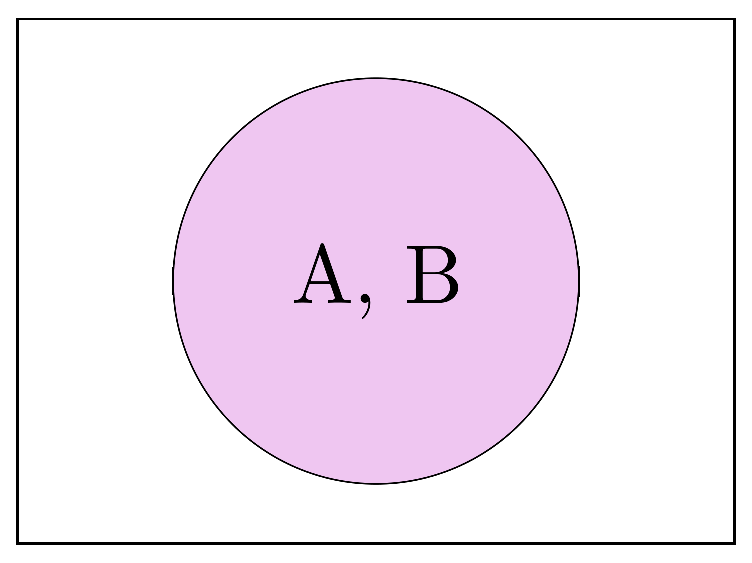
\includegraphics[width=0.2\textwidth]{discrete/sets/equal.eps}
  \end{center}
  \caption{$A=B$.}
\end{figure}
We have two ways to write an \textbf{empty set}.
We could write $\emptyset$ or $\{ \}$.

A set with only one element is called a \textbf{singleton set}.
\index{singleton set}

The set $A$ is a \textbf{subset}\index{subset} of set $B$ iff
\[ \forall x (x \in A \implies x \in B) \]
We then write $A \subseteq B$ to show that $A$ is a subset of $B$.
To demonstrate that $A$ is a subset of $B$, show that if $x$ belongs to $A$ then
it also belongs to $B$.
To show that $A$ is not a subset of $B$, that is, $A \not \subseteq B$, find a 
single element $x \in A$ such that $x \not \in B$.\footnote{\
    The symbol $\not \in$ means \emph{not in}.
}
\begin{figure}[H]
  \begin{center}
    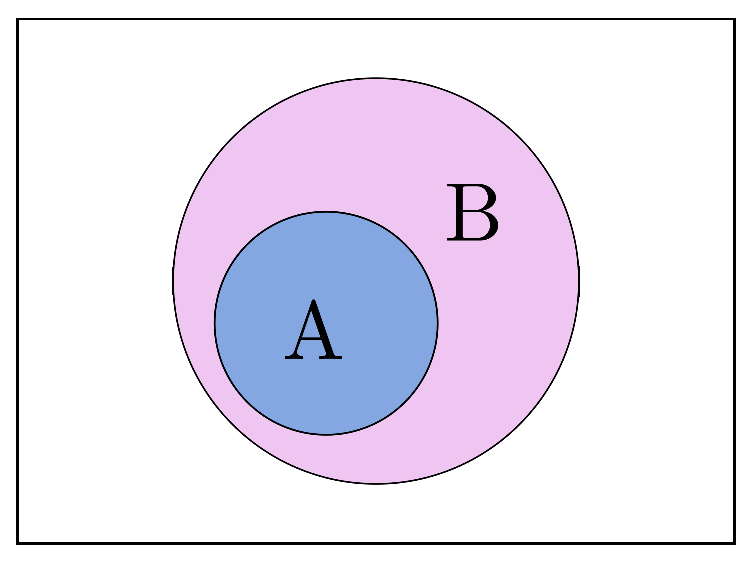
\includegraphics[width=0.2\textwidth]{discrete/sets/subset.eps}
  \end{center}
  \caption{$A\subseteq B$}
\end{figure}
If the set $A$ is a subset of the set $B$ but $A \neq B$, we write $A \subset B$ 
and say that $A$ is a \textbf{proper subset} of $B$.
That is, $A$ is a proper subset of $B$ iff
\[ \forall x (x \in A \implies x \in B) \land \exists x (x \in B \and x \not \in A). \]
This means, if the element $x$ exists in set $A$, then it also exists in set 
$B$, but there is at least one element $x$ in $B$ that is not in $A$.

\subsection{Set Operations}

For a set $A$ and a set $B$, the following operations apply:

The \textbf{cartesian product} of $A$ and $B$, denoted $A \times B$, is the set of
all ordered pairs $(a, b)$ where $a \in A$ and $b \in B$. Hence,
\[ A \times B = \big\{ (a,b) | a \in A \land b \in B \big\} \]

\begin{ex}
  Find $A \times B$ when $A = \{ 1,2 \} $ and $B = \{ a, b, c\} $.
  \begin{sol}
    \[A \times B = \big\{(1,a),(1,b),(1,c),
    (2,a),(2,b),(2,c)\big\}\]
  \end{sol}
\end{ex}

The \textbf{intersection}\index{intersection} of $A$ and $B$, denoted 
$A \cap B$,
is the set containing those elements in both $A$ and $B$, but not just one.
If the intersection of $A$ and $B$ is $\emptyset$, we say the two sets are 
\textbf{disjoint}.\index{disjoint}
\[ A \cap B = \big\{ x \in A | x \in B \big\}\]
\begin{figure}[H]
  \begin{center}
    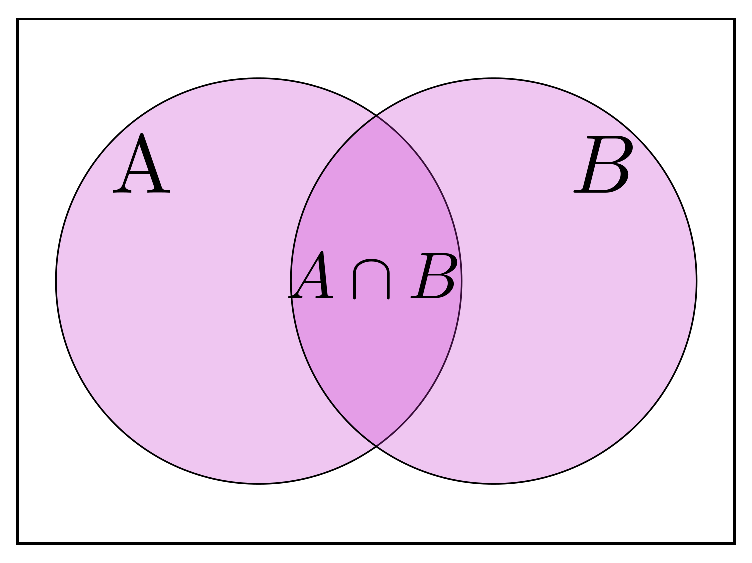
\includegraphics[width=0.2\textwidth]{discrete/sets/intersection.eps}
  \end{center}
  \caption{$A\cap B$}
\end{figure}The \textbf{union}\index{union} of $A$ and $B$, denoted $A \cup B$,
is the set containing all elements in either or both $A$ and $B$.
\[ A \cup B = \big\{ x | x \in A \lor x \in B \big\}\]
\begin{figure}[H]
  \begin{center}
    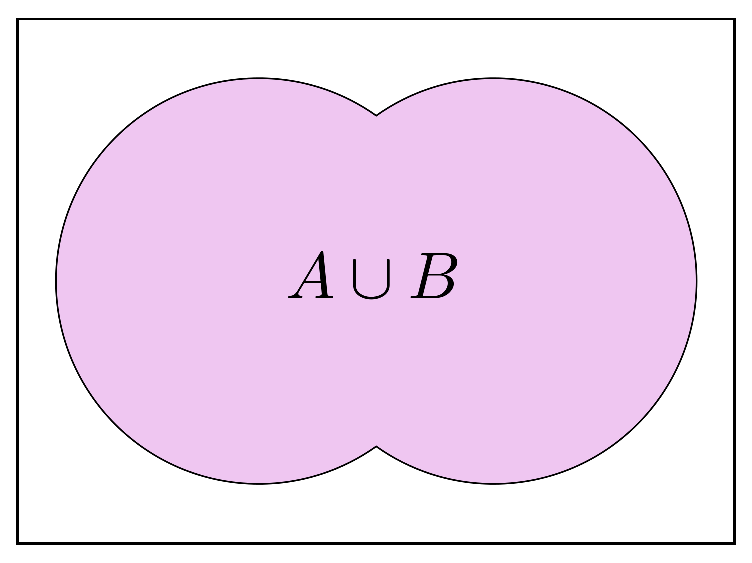
\includegraphics[width=0.2\textwidth]{discrete/sets/union.eps}
  \end{center}
  \caption{$A \cup B$}
\end{figure}
The \textbf{complement}\index{complement} of $A$ and $B$, denoted $A \setminus B$,
is the set containing those elements in $A$ but not in $B$.
It is sometimes called the \emph{component of $B$ with respect to $A$}.
This phrasing is used because the difference of $A$ and $B$ is different from the difference of $B$ and $A$.
\[ A \setminus B = \big\{ x \in A \big| x \not\in B \big\} \]

The \textbf{absolute complement}\index{absolute complement}
of $A$ is denoted $A^c$, and exists only if a universal set\footnote{A set containing all sets, including itself.}
$\mathbf{U}$ is defined, and is found by
\[ A^c = \mathbf{U} \setminus A.\]

\begin{table}
  \centering
    \begin{tabular}{>\(l<\) r}
      \textbf{Proposition} & \textbf{Name} \\ \hline\noalign{\smallskip}
      A \cap U = A & \multirow{2}{*}{identity laws} \\
      A \cup \emptyset = A \\\hline
      A \cup U = U & \multirow{2}{*}{domination laws} \\
      A \cap \emptyset = \emptyset \\\hline
      A \cup A = A & \multirow{2}{*}{idempotent laws} \\
      A \cap A = A \\\hline\noalign{\smallskip}
      \big(A^c\big)^c=A & involution law \\\noalign{\smallskip}\hline
      A \cup B = B \cup A & \multirow{2}{*}{commutative laws} \\
      A \cap B = B \cap A \\\hline
      A \cup (B \cup C) = (A \cup B) \cup C & \multirow{2}{*}{associative laws} \\
      A \cap (B \cap C) = (A \cap B) \cup C\\\hline
      A \cup (B \cap C) = (A \cup B) \cap (A \cup C) & \multirow{2}{*}{distributive laws} \\
      A \cap (B \cup C) = (A \cap B) \cup (A \cap C) \\\hline\noalign{\smallskip}
      \big(A \cup B\big)^c = A^c \cap B^c & \multirow{2}{*}{DeMorgan's laws} \\
      \big(A \cap B\big)^c = A^c \cup B^c \\\hline
      A \cup (A \cap B) = A & \multirow{2}{*}{absorbtion laws} \\
      A \cap (A \cup B) = A \\\hline
      A \cup A^c = U& \multirow{2}{*}{complement laws} \\
      A \cap A^c = \emptyset
    \end{tabular}
  \caption{Useful set identities.}
  \label{tab:setidentities}
\end{table}


\section{The Well-Ordering Principle}\index{well-ordering principle}
The \textbf{well-ordering principle} states that
\begin{theorem}
Every nonempty set of nonnegative integers has a smallest element.
\label{thm:wellordered}
\end{theorem}
We can use this to prove propositional statements associated with universal quantifiers.

To prove that
\[ \forall n \in \mathbb N \big( P(n)\big) \]
First, we define a set $C$ such that
\[ C : : = \big\{ n \in \mathbb N^+ \big| \neg P(n) \big\} \]
That is, we define the set $C$ to be the set of integers for which $P(n)$ is false.
We assume that this set is nonempty---that is, there is at least one nonnegative integer for which $P(n)$ is false.
By the well-ordering principle, there is a smallest element, $n$, in $C$.
From this, we reach a contradiction.
For example, we could show that $n$ can be used to find an element smaller than itself.
Now, we conclude that the set $C$ must be empty.

\begin{ex}
  Prove that the sum of all integers from $1$ to $n$ is \[\frac{n(n+1)}{2}.\]

  In basic algebraic notation, we could write this sum as
  \[1 + 2 + 3 + \cdots + n \]
  But we have a way of simplifying this using something called \textbf{sigma notation}\index{sigma notation}.
  We would write it as follows:
  \[1+2+3+\cdots+n  \sum_{1}^n \frac{n(n+1)}{2} \]
  \begin{proof}
    Now, we define a set $C$ such that
    \[ C : : = \bigg\{ n \in \mathbb N \big| \sum_{i=1}^n i \neq \frac{n(n+1)}{2}\bigg\}\]
    By the \emph{well-ordering principle}, $C$ has a smallest element, which we will call $c$.
    Since $c$ is the smallest counterexample,
    \[\sum_{i=1}^n = \frac{n(n+1)}{2}\]
    holds for all $n<c$ but not for $n=c$. So, that sum should hold for $c-1$:
    \begin{align*}
      1+2+3+\cdots+(c-1)&=\frac{(c-1)\big[(c-1)+1\big]}{2}\\
      1+2+3+\cdots+(c-1)&=\frac{(c-1)c}{2}\\
      1+2+3+\cdots+(c-1)&=\frac{c^2-c}{2}\\
      \intertext{Now, we add $c$ to both sides.}
      1+2+3+\cdots+(c-1)+c&=\frac{c^2-c}{2}+c\\
      \intertext{Simplify.}
      1+2+3+\cdots+(c-1)+c&=\frac{c^2-c}{2}+(c)\left(\frac{2}{2}\right)\\
      1+2+3+\cdots+(c-1)+c&=\frac{c^2-c+2c}{2} \\
      1+2+3+\cdots+(c-1)+c&=\frac{c^2+c}{2} \\
      \intertext{Factor out $c$ from the right-hand side.}
      1+2+3+\cdots+(c-1)+c&=\frac{c(c+1)}{2} \\
    \end{align*}
    Which means that
    \[\sum_{i=1}^n = \frac{n(n+1)}{2}\]
    holds for $c$, which contradicts our definition of $C$. Therefore $P(n)$ holds for all  $n \in \mathbb N$.
  \end{proof}
\cite{mcsfull}
\end{ex}

A few theorems come from the \emph{well-ordered principle}:\footnote{Proofs will come. From \cite[29]{mcsfull}.}
\begin{theorem}
  Any set of integers with a lower bound is well-ordered.
\end{theorem}
\begin{theorem}
  Any nonempty set of integers with an upper bound has a maximum integer.
\end{theorem}

%\chapter{Recursion}\index{recursion}

\section{Recursive Definitions}

\begin{defn}\index{recursive form}
  \textbf{Recursive form} defines a set, an equation, or a process by defining a starting set or a value and giving a rule for continuing to build the set, equation, or process based on previously defined terms.
\end{defn}

The key for recursion is the \emph{rule for continuing to build} the set, equation, or process. This is what allows us to do the new element, new equation, or new process based on previously defined terms.

A recursive definition has two parts.

\begin{defn}
  In the \textbf{basis step}\index{basis step}, we must define values for some finite number of
  elements. For sets, we state the \emph{basic building blocks}\index{basic
  building blocks} of the set. for functions, state the values of the function
  on the basic building blocks.
\end{defn}
\begin{defn}
  The remaining elements in the recursive definition are defined by the
  \textbf{recurrence relation}\index{recurrence relation}. For sets, we show how
  to build new things from the old with some basic construction rules. For
  functions, we show how to compute the value of a function on the new elements
  of that set.
\end{defn}

\subsection{Recursively Defined Functions}\index{functions, recursively defined}

Let us create a recursive definition of the function $F$, defined on nonnegative integers. To give a recursive definition of $F$:
\begin{enumerate}\item \emph{Basis}. Specify F(0).
    \item \emph{Recursive step}. Give a rule for defining $F(n+1)$ from $F$ evaluated at smaller values.
\end{enumerate}
\begin{ex}
  \begin{align*}
    f(0) &= 1 \\
    f(n) &= f(n-1) +2
  \end{align*}
\end{ex}
\begin{ex}
  \begin{align*}
    g(0) &= 1 \\
    g(k+1) &= g(k)+2
  \end{align*}
\end{ex}
\begin{ex}
  \begin{align*}
    a_0 &= 1 \\
    a_n &= a_{n-1}
  \end{align*}
\end{ex}
\begin{ex}
  Find the recursive form of $n!$, the function given by
  \begin{equation}\label{eq:nfact}
   n!=\prod_{k=1}^n k \
  \end{equation}
  \begin{figure}[h]
    \begin{center}
      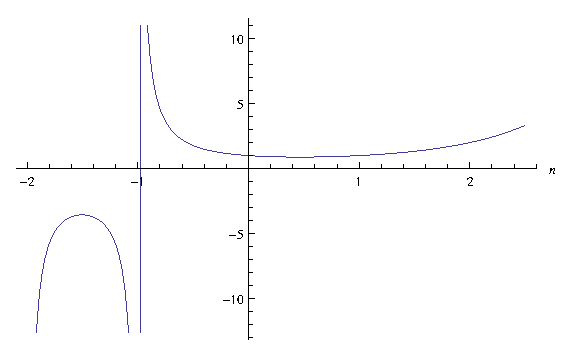
\includegraphics{discrete/recursion/nfact.eps}
    \end{center}
    \caption{A plot of $n!$. Its behavior is much harder to describe in the
    negatives, so we normally just treat it as having a domain of $n \geq 0$.}
    \label{fig:nfact}
  \end{figure}
  \begin{sol}
    The basis step in either the \emph{closed form} or \emph{recursive form}
    definition for $n!$ is that $0!=1$. In equation \eqref{eq:nfact}, it is implied
    under the convention that the product of no numbers at all is
    one\footnote{This is called the \textbf{empty product} or \textbf{nullary
    product}, and is responsible for providing the \emph{multiplicative
    identity} $1$.}

    So in order to define a recursive form for $n!$, we must start with the
    definition:
    \begin{equation}
      f(n) =
      \begin{cases}
        1 & \text{if }n=0
      \end{cases}
    \end{equation}

    Now that we have the basis step, to get the \emph{recursive step} we will
    look at a few instances of the factorial function:
    \begin{align*}
      f(0) &= 1 \\
      f(1) &= 1 \\
      f(2) &= 2 \\
      f(3) &= 6 \\
      f(4) &= 24 \\
      f(5) &= 120 \\
      & \vdots
    \end{align*}
    If we are careful, we'll notice that we can factor a $n$ from our result on
    each instance.
    \begin{align*}
      f(1) &= 1\cdot1 \\
      f(2) &= 2\cdot1 \\
      f(3) &= 3 \cdot 2 \\
      f(4) &= 4 \cdot 6 \\
      f(5) &= 5 \cdot 24 \\
      &\vdots
    \end{align*}
    We notice that $f(n)$, for any $n > 1$, is given by $n$ times the term
    before it. By writing this out, we get our \emph{recursive definition for
    factorials}.
    \begin{equation}
      f(n) =
      \begin{cases}
        1 & \text{if }n=0 \\
        n \times f(n-1) & \text{if }n > 0
      \end{cases}
    \end{equation}
    As is the case with factorials, \emph{recursive form} often offers the
    advantage that it is very intuitive for humans to understand. Its downside is
    that it is very seldom computationally faster than its \emph{closed-form}
    alternative. For this reason, we should attempt to find closed-form
    solutions to recursive definitions where possible or necessary.

    Generally speaking, given a recursive function on a test, we should be able to find a
    closed-form representation and vice-versa.
  \end{sol}
\end{ex}
\begin{ex}
  Find a recursive definition of the \textbf{Fibonacci sequence}\index{Fibonacci
  sequence}:
  \[ 1, 1, 2, 3, 5, 8 13, 21, 34, \ldots \]
  \begin{figure}[h]
    \begin{center}
      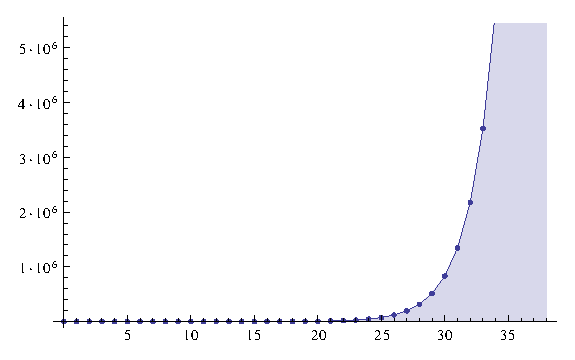
\includegraphics{discrete/recursion/fibonacci.eps}
    \end{center}
    \caption{A plot of the Fibonacci sequence.}
    \label{fig:fibonacci}
  \end{figure}

  The Fibonacci sequence is often explained using the analogy of rabbits on an
  island.
  \begin{quote}
    ``A young pair of rabbits (one for each sex) is placed on an island. After
    they are 2 months old, each pair of rabbits produces another pair each month.
    The number of pairs of rabbits after $n$ months is $f(n)$.''
  \end{quote}
  \begin{sol}
    Notice that we need \textbf{two} initial conditions to define this
    recurrence relation.
    \begin{equation}
      f(x) =
      \begin{cases}
        1 & \text{for }0 \leq x \leq 1 \\
        f(n) + f(n-1) &\text{for } x > 1
      \end{cases}
    \end{equation}
  \end{sol}
  \begin{note}
    This definition requires two initial conditions. It is very important in recursive definitions to have the right number of initial conditions.
  \end{note}
\end{ex}
%\begin{ex}
%  Give a recursive definition of
%  \[ F(n) = a^n \]
%
%  \begin{tabular}{ll}
%    $f(0)=a^0=1$ & basis \\
%    $f(n)=a\cdot f(n-1)$& recursion \\
%  \end{tabular}
%  \begin{note}
%    \[f(n)=a^n=\underbrace{a \cdot a \cdot a \cdot \dots a}_{n}\]
%
%    \[f(n-1)=a^{n-1}=\underbrace{a \cdot a \cdot a \cdot \dots a}_{n-1}\]
%  \end{note}
%\end{ex}
%\begin{ex}
%  Give a recursive definition of
%  \[ F(n) = \sum^{n}_{k=0} a_k \]
%
%  \begin{tabular}{ll}
%    $f(c)=a_0$ & basis \\
%    $f(n)=f(n-1)+a_n$ & recursion \\
%  \end{tabular}
%  \begin{note}
%    \[ F(n) = \sum^{n}_{k=0} a_k=a_0+a_1+\dots+a_{n-1}+a_n \]
%  \end{note}
%\end{ex}
%
%\begin{comment}
%\begin{ex}
%  \begin{tabular}{ll}
%    Basis. & $f(0)=100,000=A$ \\
%    Recursion. & $f(k)=f(k-1)+f(k-1)*4\%$ \\
%    & $f(k) = (1+\alpha)(f(k-1))$ \\
%  \end{tabular}
%  \begin{tabular}{ll}
%
%  \end{tabular}d
%  \end{ex}
%\end{comment}
%
%  Mathematical induction is a way to varify the correctness of a recursive definition.
%
%  \begin{ex}
%    \begin{align*}
%      a_1&=1 \\
%      a_n&=2a_{n-1}+1 \text{ for all integers n $\geq 2$}
%      \intertext{Then prove by induction:}
%      a_n&=2^n-1 \text{ for all } n \geq 1
%    \end{align*}
%    \begin{tabular}{ll}
%      & $a_1=2^1-1=1=a_1 \text{ by recursion}$\\
%      & If $a_n=2n-1$, then $a_{n+1}=2^{n+1}-1$. \\
%      & assume $a_n=2^n-1$ \\
%      & $a_{n+1}=2a_n+1=2(2^n-1)+1$ \\
%      & $= 2 \cdot 2^n -2 +1 = 2^{n+1}-1$
%    \end{tabular}
%  \end{ex}
%
%\section{Recursive Algorithms}
%
%Recursive algorithms are only used because certain algorithms are recursive in nature. Recursion does not save any computational power. For most algorithms, we can define a non-recursive version. However, sometimes it is inconvenient to find a non-recursive equivalent to a recursive algorithm.
%
%A recursive algorithm is one which calls itself to sove ``smaller'' versions of an input problem. Some algorithms are recursive in nature, like the binary search or Fibonacci sequence.
%
%The current status of the algorithm is placed on the \emph{stack}. A stack is a data structure from which entries can be added and deleted only from one end.
%
%\begin{verbatim}
%  procedure factorial(n)
%    if n < 0 return 'error'
%    if n = 0 the nreturn 1
%    else
%      return (n*factorial(n-1))
%\end{verbatim}
%
%Say we want to calculate $f(3)$.
%
%\begin{align*}
%  f(3)=3 \cdot &f(2)&&\\
%  &\to f(2) = 2 \cdot f(1)&\\
%  &&\to f(1)=1\cdot &f(0)\\
%  &&&\to f(0)=1
%\end{align*}
%
%
%

\chapter{Counting}

We can use counting techniques to determine the complexity of an algorithm.
Counting is very important not only for computer science but also for any job.
For example, counting problems are common in job interviews to see how a potential employee reacts.

Counting, ultimately, is a very simple theoretical process governed by some basic rules.

\section{Rules of Counting}

\subsection{The Sum Rule}\index{sum rule for counting}
  If a first task can be done in \(n_1\) ways and a second task can be done in \(n_2\) ways,
  and if these tasks cannot be done at the same time, then there are \(n_1+n_2\) ways to do either task.

  In set notation: if \(A\) and \(B\) are \emph{disjoint}, then \(|A \cup B|=|A|+|B|\).

\subsection{The Product Rule}\index{product rule for counting}

Suppose that a procedure can be broken down into two tasks.
If there are \(n_1\) ways to do the first task and 
\(n_2\) ways to do the second task
\emph{after} the first task has been done,
n there are \(n_1n_2\) ways to do the procedure.

In set notation:
\[|A \times B| = |A||B| \]

\subsection{Examples}

\begin{ex}
  Let \(D = \{x, y, z\}\). Let \(R=\{1,2,3,4,5\}\).
  \begin{itemize}
    \item[a) ] How many functions are there from \(D\to R\)?
    \item[b) ] How many \emph{one-to-one} functions are there?
    \item[c) ] How many onto functions are there?
  \end{itemize}
  \begin{sol}
    We only have two rules for counting right now.
    For the product rule, we must assume we are going to define mapping for \(x\), then for \(y\), then for \(z\).
    With the sum rule, then we can define mapping for \(x\), or \(y\), or \(z\).

    Then we go back to ``how do we define the function?'' Do we have to find a mapping for every element in the domain?

    Yes. By definition of functions, we must.


    \begin{itemize}
      \item[a) ] There are \(5 \times 5 \times 5\) possible mappings from \(D \to R\).
      \item[b) ] \(5\times4\times3\).
      \item[c) ] It is impossible for the function to be onto. There are not enough elements in the domain to have values in the range to map to them.:w
    \end{itemize}
  \end{sol}
\end{ex}
\begin{ex}
  A typical PIN is a sequence of any four numbers chosen form the 26 letters and the ten digits.
  \begin{itemize}
  \item[a) ] How many different PINs are possible if repetition is allowed?
    \item[b) ] What if repetition is not allowed?
  \end{itemize}
  \end{ex}
\begin{ex}
  The ASCII character set is represented by 7 binary bits. How many characters are there in the set?
  % \begin{sol}
  %  We have to make seven choices in sequence to come up with an ASCII character.
  %  For each choice, we have two choices.
  % \end{sol}
\end{ex}
\begin{ex}
  Count the number of binary bit strings of length 4 or less.
\end{ex}
\begin{ex}
  A student can choose a computer project from one of three lists. The three lists contain 10, 20, or 30 possible projects. There is no overlap among that list. How many projects are there to choose from?
  \begin{sol}
    \[10+20+30 \text{ projects}\]
  \end{sol}
\end{ex}

\section{The Pidgeonhole Problem}\index{pidgeonhole problem}
\begin{quote}
  A flock of 13 pideons roosts in a set of 12 pidgeonholes. One of the
  pidgeonholes must have more than one pidgeon.
\end{quote}
If $k$ is a positive integer and $k+1$ objects are placed into $k$ boxex, then
at least one box must have more than one object.
\begin{proof}
  We can prove this by contradiction. Suppose all of the pidgeons fit in to $k$
  boxes exclusively. Therefore, there must be $k$ pidgeons, which is not equal
  to $k+1$.
\end{proof}
\begin{corollary}
  A function $f$ from a set with $k+1$ elements to a set with $k$ elements is
  not \emph{one-to-one}.
  \begin{proof}
    Say we have eight boxes. We want to divide the objects evenly among the
    boxes, so we place $2$ in each box. The number of boxes over the number of
    elements is equal to $2$ objects per box.

    For nine boxes, we must take the ceiling function of $9/4$ and find 3.
  \end{proof}
\end{corollary}
\begin{theorem}
  \label{th:pidgeonhole}
  If $N$ objects are placed into $k$ boxes, then there is at least one box
  containing at least $N/K$ objects.
\end{theorem}
\begin{ex}
  Among 100 people there are at least [100/12]=9 who were born in the same
  month.
\end{ex}
\begin{ex}
  How many cards must be selected from a standard deck of 52 cards to guarantee
  that at least three cards of the same suit are selected. After generalizing
  the pidgeonhole problem, we find that at least one box contains at least
  $[N/4]$ cards. At least three cards of one suit are selected 
\end{ex}
\section{Combination Rule}

For the addition rule, we know the values and don't know the positions.
Where we know the position and don't know the values, we use the combination
rule to solve the problems.

For the rule of products, things are more general. We can select the same
elements, and we are determining value rather than location.

\begin{ex}
  How many bit strings of length $100$ have at least $2$ ones?
  \begin{sol}
    The solution is given by the combination rule:
    \[ C(100 2) \]
    For exactly 3 ones, we do
    \[ C(100, 3) \]
    One hundred $1$s:
    \[ C(100,100) \]
    Or
    \[ C(100, 2) + C(100, 3),+ \cdots + C(100,100) \]
    We can do this using the combination rule as follows:
    \[ 2^{100} - C(100,0) - C(100,1) \]
    which is the total number of bit strings with at least 2 ones.
  \end{sol}
\end{ex}

\section{Counting the Complement}

This is an applicaiton of the set decomposition principle, which states that the
total number of objects is equal to the number of objects that have a certain
property plus the number of objects that do not have the property.
\begin{ex}
  Passwords of lenght 8 are made of lowercase letters and decimal digits. How
  many of such passwords contain at least one decimal digit?
  
  In the past, we solved this as follows:
  \[ (26+10)^8 = \text{ number of passwords with more than one digit} + 26^8 \]

  The combination rule will tell us:location of digit -> value of digit ->
  value of letters


  Number of passwords with one digit:
  \[ C(8,1) \times 10 \times 26^7 \]
  The number of passwords with two digits:
  \[ C(8,2)\times10^2\times26^6 \]
  And so on. The sum of these numbers provides our answer.
\end{ex}

\section{The Binomial Theorem}
\begin{ex}
  Find the expansion of
  \[(x+y)^2,\, (x+y)^3\]
  \begin{sol}
    \[(x+y)^2 = x^2 + 2\times y+ y^2\]
    That is to say,
    \[ C(2, 0)+ C(2, 1)+ C(2,2) \]
    For
    \[(x+y)^3\]
    we get
    \begin{align*}
      (x+y)^3&=C(3,0)+C(3,1)+C(3,2)+C(3,3) \\
      &= x^3 + 3x^2 y + 3 x y^2 + y^3
       &= (x+y)(x+y)(x+y)
    \end{align*}
  \end{sol}
\end{ex}
This gives us the \textbf{binomial theorem}.
\[ (x+y)^n = \sum^n_{j=0} C(n, j)x^{n-j}y^j \]
\begin{ex}
  What is the coefficient of $x^{25}y^{75}$ in the expansion of $(2x-5y)^{100}$?
  \begin{sol}
    Let $2x=a$ and $5y =b$.
    \[ (a+b)^n= \sum^n_{j=0} C(n,j) a^{n-j} b^j \]
    Now we solve for the variables. We know $a$, $b$, and $n$, so we must solve for
    $j=75$.
    Now, we put together our sum.
    \[ C(100,75)(2x)^{100-75}(-5y)^{75} \]
    \[ = C(100,75) 2^{25} \cdot x^{25} \cdot (-5)^{75} \cdot y^{75} \]
    Which makes our answer
    \[ C(100, 75) \cdot 2^{25}\cdot(-5)^{25}\]
  \end{sol}
\end{ex}
\begin{homework}
  Section $6.3$ (p.413): $17,20,33,34,37$.
  Section $6.4$ (p.421): $3, 5, 9$.

  On Monday, we will get the even numbered answers for sections $6.1-6.4$,
  around six or seven questions. We will also receive the review question
  answers. This homework will be due on Tuesday, along with a quiz on counting.
  Review the self-assessment on the counting sction.
\end{homework}

